%%%%%%%%%%%%%%%%%%%%%%%%%%%%%%%%%%%%%%%%%%%%%%%%%%%%%%%%%%%%%%%%%%%%%%
% Lớp 12 | Nguyên hàm, tích phân | Ứng dụng thực tế và hình học của tích phân
% Dạng 2D4?3-4: Thể tích tính theo mặt cắt 𝑆(𝑥)
% Số câu: 17  (sinh tự động bởi tach_cau.py; từ nay thầy sửa trực tiếp file này)
%%%%%%%%%%%%%%%%%%%%%%%%%%%%%%%%%%%%%%%%%%%%%%%%%%%%%%%%%%%%%%%%%%%%%%

%%%%%%%%%%%%%%%% TRẮC NGHIỆM 4 PHƯƠNG ÁN %%%%%%%%%%%%%%%%

% nguồn: Phan1_Lop_12_Dai_so_Chuong_4
\begin{ex}%[2D4N3-4]%[ma:11613aa2]
	Trong không gian $Oxyz$, cho vật thể $T$ giới hạn bởi hai mặt phẳng có phương trình $x=a$ và $x=b$ $(a<b)$. Cắt vật thể $T$ bởi một mặt phẳng vuông góc với trục $Ox$ tại điểm có hoành độ bằng $x$ $(a \leq x \leq b)$, ta  được thiết diện có diện tích bằng $S(x)$. Khi $S(x)$ là một hàm liên tục trên đoạn $[a;b]$, thể tích $V$ của vật thể $T$ được tính theo công thức nào sau đây?
	\begin{center}
		\begin{tikzpicture}[scale=0.8,font=\footnotesize,line join=round,line cap=round,>=stealth]
				\draw plot[smooth,tension=.65] coordinates{(1,2) 
					(2.5,2.3) 
					 (3.5,2.2)};
				\draw[dashed] plot[smooth,tension=.65] coordinates{(3.5,2.2) 
					 (4,2)};
				\draw  plot[smooth,tension=.65] coordinates{(4,2)
					(5,2.2) 
					 (5.5,2.1)};
				 \draw[dashed] plot[smooth,tension=.65] coordinates{(5.5,2.1)
					(6,2)}; 
				\draw  plot[smooth,tension=.65] coordinates{(1,1)
					(2.3,0.5) 
					 (3.5,0.8)};
				\draw[dashed] plot[smooth,tension=.65]  coordinates{(3.5,0.8)
					 (4,1)};
				\draw  plot[smooth,tension=.65] coordinates{(4,1)
					 (5,0.7)
					 (5.5,0.8)};
				 \draw[dashed] plot[smooth,tension=.65] coordinates{(5.5,0.8)
					 (6,1)};
				\draw[dashed] (1,1) arc (-90:90:.2 and  0.5);
				\draw  (1,2) arc (90:270:.2 and 0.5);
				\draw[dashed] (4,1) arc (-90:90:.2 and 0.5); 
				\draw (4,2) arc  (90:270:.2 and 0.5);
				\draw (6,1) arc (-90:270:.2 and  0.5);
				\fill[pattern=north east lines] (4,1) arc (-90:90:.2 and 0.5)--(4,2)  arc (90:270:.2 and 0.5)--cycle;
				\draw (-.5,0)--(0.5,0) 
					(1,0)--(3.5,0) 
					(4,0)--(5.5,0); 
				\draw[dashed]  (0.5,0)--(1,0)
					 (3.5,0)--(4,0)
					 (5.5,0)--(6,0);
				\draw[->] (6,0)--(7,0)  node[below]{$x$};
				 \draw[->] (0,0)--(-2,-1) node[below]{$y$};
				 \draw[->] (0,0)--(0,3.5) node[right]{$z$};
				\draw  (0.5,-1)--(0.5,3)--(1.5,3.5)--(1.5,2.2)
					 (1.5,.8)--(1.5,-0.5)--(0.5,-1);
				 \draw[dashed](1.5,2.2)--(1.5,.8);
				 \draw[dashed] (1,1)--(1,0) node[below]{$a$};
				\coordinate  (A) at (0.5,3);
				\coordinate (B) at  (1.5,3.5);
				\coordinate (C)  at (1.5,2.2);
				\draw pic[draw,angle eccentricity=1.6,angle radius=0.5cm]{angle=A--B--C}; 
				\draw (1.3,3.2)  node {$P$};
				 \draw (3.5,-1)--(3.5,3)--(4.5,3.5)--(4.5,2)
					 (4.5,1)--(4.5,-0.5)--(3.5,-1);
				\draw[dashed](4.5,2)--(4.5,1); 
				\draw[dashed] (4,1)--(4,0) node[below]{$x$}; 
				 \coordinate (D) at (3.5,3);
				\coordinate (E) at  (4.5,3.5);
				 \coordinate (F) at (4.5,2);
				\draw  pic[draw,angle eccentricity=1.6,angle radius=0.5cm]{angle=D--E--F};
				 \draw (4.3,3.2) node {$R$};
				\draw (5.5,-1)--(5.5,3)--(6.5,3.5)--(6.5,-0.5)--(5.5,-1); 
				 \draw[dashed] (6,1)--(6,0) node[below]{$b$};
				\coordinate (G)  at (5.5,3);
				 \coordinate (H) at (6.5,3.5);
				\coordinate (K) at  (6.5,-0.5);
				 \draw pic[draw,angle eccentricity=1.6,angle radius=0.5cm]{angle=G--H--K}; \draw (6.3,3.2) node {$Q$};
				\draw (0,-.3)  node {$O$};
				\fill (0,0) circle  (1pt);
				\draw[->] (4,1.5)--(4.7,1.7)  node[right] {$S (x)$};
			\end{tikzpicture}
	\end{center}
	 \choice
		{\True $V=\displaystyle\int_a^b S(x)\,\mathrm{\,d}x$} 
		{$V=\pi\displaystyle\int_a^b S(x)\,\mathrm{\,d}x$} 
		{$V=\displaystyle\int_b^a S(x)\,\mathrm{\,d}x$} 
		{$V=\pi\displaystyle\int_a^b [S(x)]^2\,\mathrm{\,d}x$} 
	 \loigiai{
	Thể  tích $V$ của vật thể $T$ được tính theo công thức $V=\displaystyle\int_a^b S(x)\,\mathrm{\,d}x$.}
\end{ex}

% nguồn: Phan1_Lop_12_Dai_so_Chuong_4
\begin{ex}%[2D4N3-4]%[ma:1be14dfd]
	Cho một vật thể trong không gian $Oxyz$. Gọi $\mathcal{B}$ là phần vật thể giới hạn bởi hai mặt phẳng vuông góc với trục $Ox$ tại các điểm có hoành độ $x=a, x=b\,(a<b)$. Một mặt phẳng vuông góc với trục $Ox$ tại điểm có hoành  độ $x$ cắt vật thể theo mặt cắt có diện tích là $S(x)$. Giả sử $S(x)$ là hàm số liên tục trên đoạn $[a; b]$. Khi đó, thể tích của phần vật thể $\mathcal{B}$ được tính bởi công thức là
	\choice 
		 {$\pi \displaystyle\int_a^b S(x)\mathrm{\,d}x$}
		{$\pi \displaystyle\int_a^b[S(x)]^2 \mathrm{~d}  x$}
		{$\displaystyle\int_a^b[S(x)]^2 \mathrm{~d} x$} 
		{\True  $\displaystyle\int_a^b S(x)\mathrm{\,d}x$}
	 \loigiai{
		 Ta có $V=\displaystyle\int_a^b S(x)\mathrm{\,d}x$.
	 }
\end{ex}

% nguồn: Phan1_Lop_12_Dai_so_Chuong_4
\begin{ex}%[2D4N3-4]%[ma:4fc09874]
	Cho một vật thể trong không gian $Oxyz$. Gọi  $\beta$ là phần vật thể giới hạn bởi hai mặt phẳng vuông góc với trục $Ox$ tại các điểm có hoành độ $x=a$, $x=b$. Một mặt phẳng vuông góc với trục $Ox$ tại điểm có hoành độ là $x$ cắt vật thể theo mặt cắt có diện tích là $S(x)$. Giả sử $S(x)$ là hàm số liên tục trên đoạn $\left[a;b\right]$. Khi đó thể tích $V$ của phần vật thể $\beta$ tính bởi công thức là
	 \choice
		{$V=\pi\displaystyle\int_a^b S(x)\mathrm{\,d}x$} 
		 {$V=\pi\displaystyle\int_a^b S^2(x)\mathrm{\,d}x$}
		{$V=S'(x)$} 
		{\True $V=\displaystyle\int_a^b S(x)\mathrm{\,d}x$} 
	\loigiai{ 
		Theo định nghĩa, thể tích vật thể với mặt cắt vuông góc trục  $Ox$ có diện tích $S(x)$ là
		\[ 
		V=\displaystyle\int_a^b  S(x)\mathrm{\,d}x.
		 \]
	} 
\end{ex}

% nguồn: Phan1_Lop_12_Dai_so_Chuong_4
\begin{ex}%[2D4N3-4]%[ma:5bbb656e]
	Xét trong không gian $Oxyz$, tính thể tích của vật thể nằm giữa hai mặt phẳng $x=-1$ và $x=1$ biết rằng thiết diện  của vật thể bị cắt bởi mặt phẳng vuông góc với trục $Ox$ tại điểm có hoành độ $x~(-1\leq x \leq 1)$ là một hình vuông cạnh là $2\sqrt{1-x^2}$.
	\choice 
		{\True $V=\dfrac{16}{3}$} 
		{$V=\dfrac{16\pi}{3}$} 
		{$V=\dfrac{14}{3}$} 
		 {$V=\dfrac{14\pi}{3}$}
	\loigiai{ 
		Thiết diện của vật thể bị  cắt là hình vuông có cạnh là $2\sqrt{1-x^2}$ nên diện tích thiết diện là $S(x)=4\left(1-x^2\right)$.\\
		Thể tích của vật  thể là $V=\displaystyle\int_{-1}^1S(x) \mathrm{\,d}x=\displaystyle\int_{-1}^14\left(1-x^2\right) \mathrm{\,d}x=\left(4x-\dfrac{4}{3} x^3\right)\bigg|_{-1}^1=\dfrac{16}{3}$.
	 }
\end{ex}

% nguồn: Phan1_Lop_12_Dai_so_Chuong_4
\begin{ex}%[2D4H3-4]%[ma:d5721e7f]
	Tính thể tích $V$ của phần vật thể giới hạn bởi hai mặt phẳng $x=0$, $x=1$, có thiết diện bị cắt bởi mặt phẳng vuông góc với trục $Ox$  tại điểm có hoành độ $x$ thỏa mãn $0 \le x \le 1$ là một tam giác đều có cạnh bằng $x$.
	\choice 
		 {$V=\dfrac{12\pi}{5}$}
		{$V=\dfrac{12}{5}$} 
		{$V=\dfrac{\sqrt{3}}{12}$} 
		{\True$V=\dfrac{\sqrt{3}}{12}$} 
	\loigiai{Diện tích của thiết diện là  $$S(x)=\dfrac{x^2\sqrt{3}}{4}.$$
	Thể  tích vật thể là $$V=V=\displaystyle\int_{0}^{1}S(x)\mathrm{\,d}x=\displaystyle\int_{0}^{1}\dfrac{x^2\sqrt{3}}{4}\mathrm{\,d}x=\dfrac{\sqrt{3}}{12}.$$}
\end{ex}

% nguồn: Phan1_Lop_12_Dai_so_Chuong_4
\begin{ex}%[2D4H3-4]%[ma:b5910a1a]
	Khi cắt một vật thể bởi mặt phẳng vuông góc với trục $Ox$ tại điểm có hoành độ $x$, $(-2 \leq x \leq 2)$, mặt cắt là hình vuông có độ dài các cạnh là $\sqrt{4 - x^2}$. Thể tích của vật thể đã cho bằng bao  nhiêu?
	 \choice
		 {$\dfrac{2\pi}{3}$}
		{\True $\dfrac{32}{3}$} 
		{$\dfrac{32}{3} \pi$} 
		{$\dfrac{2}{3}$} 
	 \loigiai{
		Diện tích của mặt cắt hình vuông là  $S(x) = \left(\sqrt{4 - x^2}\right)^2 = 4 - x^2$.\\
		Thể tích của vật thể đã cho là là $V = \displaystyle\int_{-2}^{2} S(x) \mathrm{\,d}x  = \displaystyle\int_{-2}^{2} (4 - x^2) \mathrm{\,d}x=\dfrac{32}{3}
		$. 
	} 
\end{ex}


%%%%%%%%%%%%%%%% ĐÚNG/SAI %%%%%%%%%%%%%%%%

% nguồn: Phan1_Lop_12_Dai_so_Chuong_4
\begin{ex}%[2D4H3-4]%[ma:88ea6842]
	Cho khối chóp đều có đáy là hình vuông cạnh $L$ và chiều cao là $h$. Chọn trục $Ox$  sao cho gốc $O$ trùng với đỉnh của khối chóp và trục đi qua tâm của đáy (như hình dưới).
	\begin{center}
		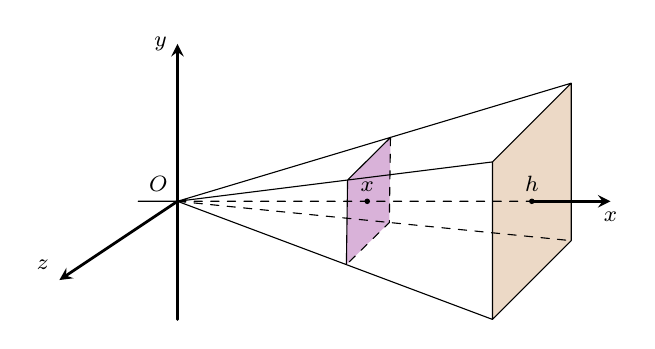
\begin{tikzpicture}[scale=.5,font=\footnotesize,line join=round,line cap=round,>=stealth]
				\begin{scope}[shift={(0,0)}]
					\fill[brown!30]  (8,1)--(10,3)--(10,-1)--(8,-3)--cycle;
					 \fill[violet!30] (5.41,1.62)--(5.38,-0.54)--(4.29,-1.61)--(4.32,0.54)--cycle;
					\draw[->,line width =  1pt] (9,0)--(11,0) node[below]{$x$};
					\draw[->,line width = 1pt] (0,-3)--(0,4) node[left]{$y$}; 
					\draw[->,line width = 1pt] (0,0)--(-3,-2) node[above  left]{$z$};
					\draw (8,1)--(10,3)--(10,-1)--(8,-3)--cycle (4.29,-1.61)--(4.32,0.54)--(5.41,1.62) 
						(0,0)--(8,-3) 
						(0,0)--(8,1) 
						 (0,0)--(10,3)
						 (-1,0)--(0,0);
					 \draw[dashed] (5.41,1.62)--(5.38,-0.54)--(4.29,-1.61)
						 (0,0)--(10,-1)
						(0,0)--(9,0); 
					 \fill (0,0) circle (1pt) node[above left]{$O$};
					\fill (4.82,0) circle (2pt) node[above]{$x$}; 
					\fill (9,0) circle (2pt) node[above]{$h$}; 
				\end{scope}
			\end{tikzpicture}
	\end{center}
	\choiceTF 
		{Đáy của khối chóp  nằm trên mặt phẳng song song với $Ox$}
		{\True Mỗi mặt phẳng vuông góc với trục $Ox$  tại điểm có hoành độ bằng $x$, $\left(0\le x\le h\right)$, cắt khối chóp theo mặt cắt là hình vuông cạnh $a$}
		{Diện tích mặt cắt là  $S(x)=\dfrac{L}{h}{x^2}$}
		{\True Thể tích  của khối chóp là $V=\dfrac{1}{3}{L^2}h$}
	 \loigiai{
		\begin{center}
			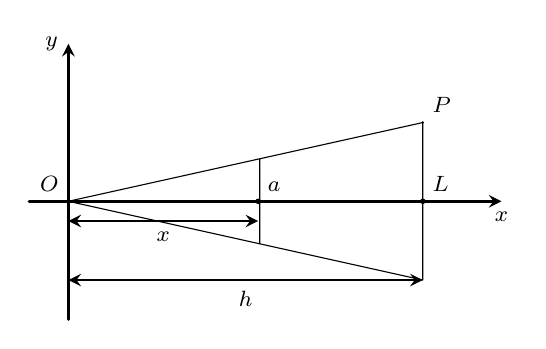
\begin{tikzpicture}[scale=.5,font=\footnotesize,line join=round,line cap=round,>=stealth]
					\begin{scope}[shift={(15,0)}]
						\draw[->,line width = 1pt] (-1,0)--(11,0) node[below]{$x$}; 
						\draw[->,line  width = 1pt] (0,-3)--(0,4) node[left]{$y$};
						\draw (0,0)--(9,2)--(9,-2)--cycle (4.86,1.08)--(4.86,-1.08); 
						\fill (4.82,0) circle  (2pt) node[above right]{$a$};
						\fill (9,0) circle (2pt) node[above right]{$L$}; 
						\draw[<->,line width = 1pt] (0,-0.5)--(4.82,-0.5) node[pos=0.5,sloped,below]{$x$}; 
						\draw[<->,line width = 1pt] (0,-2)--(9,-2)  node[pos=0.5,sloped,below]{$h$};
						 \fill (0,0) circle (1pt) node[above left]{$O$};
						\fill (9,2) circle (1pt) node[above  right]{$P$};
					\end{scope}
				\end{tikzpicture}
		\end{center}
		\begin{itemchoice}
			 \itemch Đáy của khối chóp nằm trên mặt phẳng vuông góc với $Ox$ tại $x=h$.
			\itemch Mỗi mặt phẳng vuông góc với trục $Ox$ tại điểm có hoành độ bằng $x$ $\left(0\le x\le  h\right)$, cắt khối chóp theo mặt cắt là hình vuông có cạnh là $a$.
			\itemch Theo định lí Tha-les, ta có $\dfrac{x}{h}=\dfrac{\dfrac{a}{2}}{\dfrac{L}{2}}$ suy ra $a=\dfrac{L}{h}x$.\\ 
			Do đó, diện tích của mặt cắt này  là $S(x)=\dfrac{L^2}{h^2}{x^2}$.
			\itemch Thể tích của  khối chóp này là $V=\displaystyle\int_0^h{S(x){\rm{d}}x}=\displaystyle\int_0^h{\dfrac{L^2}{h^2}{\rm}{x^2}{\rm{d}}x}=\left.\dfrac{L^2}{h^2}\cdot\dfrac{x^3}{3}\right|_0^h=\dfrac{1}{3}{L^2}h$.
		\end{itemchoice}
	 }
\end{ex}

% nguồn: Phan1_Lop_12_Dai_so_Chuong_4
\begin{ex}%[2D4V3-4]%[ma:f096d663]
	Trong không gian $Oxyz$ cho vật thể nằm giữa hai mặt phẳng $x=-1$ và $x=1$. Thiết diện của vật thể đó cắt bởi mặt  phẳng vuông góc với trục $Ox$ tại điểm có hoành độ $x$ thỏa mãn $-1\leq x \leq 1$ là một tam giác vuông cân với cạnh huyền bằng $\sqrt{1-x^2}$.
	 \choiceTF
		{\True Thiết diện tại điểm có hoành độ $x$ là tam giác vuông cân có cạnh góc  vuông là $\dfrac{\sqrt{1-x^2}}{\sqrt{2}}$}
		{Diện tích thiết diện tại điểm có hoành  độ $x$ là $S(x)=\dfrac{1-x^2}{2}$}
		{Công thức tính thể tích vật thể theo  diện tích mặt cắt $S(x)$ với $a \leq x \leq b$ là $V=\pi\displaystyle\int_a^b S(x) \mathrm{\,d}x$}
		{\True Thể tích của vật  thể đã cho là $\dfrac{1}{3}$}
	\loigiai{ 
		\begin{itemchoice}
			 \itemch \textbf{Đúng}.\\
			Tam giác vuông cân có cạnh góc vuông  là $\dfrac{\sqrt{1-x^2}}{\sqrt{2}}$.
			\itemch  \textbf{Sai}.\\
			Diện tích tam giác vuông cân có cạnh góc vuông  $\dfrac{\sqrt{1-x^2}}{\sqrt{2}}$ là $S(x)=\dfrac{1-x^2}{4}$.
			\itemch \textbf{Sai}.\\ 
			Công thức tính thể tích vật thể theo diện tích mặt cắt $S(x)$ với $a \leq x \leq b$ là $V=\displaystyle\int_a^b S(x) \mathrm{\,d}x$. 
			\itemch  \textbf{Đúng}.\\
			 Ta có $V=\displaystyle\int_{-1}^1 \dfrac{1-x^2}{4} \mathrm{\,d}x=\dfrac{1}{3}$.
		\end{itemchoice}
	} 
\end{ex}


%%%%%%%%%%%%%%%% TRẢ LỜI NGẮN %%%%%%%%%%%%%%%%

% nguồn: Phan2_Lop_12_Dai_so_Chuong_4
\begin{bt}%[2D4H3-4]%[ma:70017bfc]
	\immini{Một chiếc lều mái vòm có hình dạng như hình bên. Nếu  cắt lều bằng mặt phẳng song song với mặt đáy và cách mặt đáy một khoảng $x$ (m) ($0 \le x \le 3$) thì được hình vuông có cạnh $\sqrt{9-x^2}$. Thể tích của chiếc lều bằng bao nhiêu m$^3$? (Làm tròn kết quả đến hàng phần mười)
	\shortans{18} 
	}{\begin{tikzpicture}[line join = round,line cap=round,>=stealth,font=\footnotesize,scale=0.7]
		 \path
			(0,0)  coordinate (A)
			 ($(A)+(0.3,2.5)$) coordinate (A1)
			(4,0)  coordinate (B)
			($(B)+(-0.5,2.5)$) coordinate  (B1)
			 (-2,-2) coordinate (D)
			($(D)+(0.5,2.5)$) coordinate (D1) 
			($(B)+(D)-(A)$) coordinate  (C)
			($(B1)+(D1)-(A1)$) coordinate  (C1)
			($(A)!1/2!(C)$)  coordinate (O)
			 ($(A1)!1/2!(C1)$) coordinate (O1)
			($(O)+(0,4.5)$) coordinate (S); 
		\fill[yellow!30] (D)..controls +(90:0.5) and +(-110:0.5)..(D1) 
			--(D1)..controls +(70:3) and  +(-170:0.1)..(S)
			 .. controls +(-10:0) and +(130:1.5)..(B1)
			.. controls +(-50:0.1)  and +(90:2)..(B) --(C)--(D);
		\fill[yellow] (D1)--(A1)--(B1)--(C1)--(D1); 
		\fill (O)  circle (1.5pt)
			(O1) node[above left]{$x$} circle  (1.5pt);
		 \draw[dashed] (D)--(A)--(B)
			(S)--(O); 
		\draw (D)--(C)--(B) 
			 (C1)--(B1) node[pos=0.5,below,rotate=47,scale=1.5,font=\scriptsize]{$\sqrt{9-x^2}$}
			($(D)!1/2!(C)+(0,-0.5)$); 
		\draw 
			(D)..controls +(90:0.5)  and +(-110:0.5)..(D1)
			 --(D1)..controls +(70:3) and +(-170:0.1)..(S)
			(C)..controls +(95:2) and +(-80:0.)..(C1) 
			(C1)..controls+(100:3) and  +(-70:0)..(S)
			(B)..controls+(90:2) and  +(-50:0.1)..(B1)
			(B1)..controls+(130:1.5) and  +(-10:0.)..(S)
			(D1)--(C1)--(B1); 
		\draw pic[draw,angle  radius=3mm] {right angle = A1--D1--C1};
		 \draw[dashed]
			 (A)..controls+(90:1.5) and +(-110:0.1)..(A1)
			 (A1)..controls+(70:0.75) and +(-130:0.1)..(S)
			(D1)--(A1)--(B1); 
	\end{tikzpicture}
	 }
	\loigiai{ 
		\begin{center}
			\begin{tikzpicture}[line join = round,line cap=round,>=stealth,font=\footnotesize,scale=0.7]
					 \path
						(0,0)  coordinate (A)
						($(A)+(0.3,2.5)$) coordinate  (A1)
						(4,0)  coordinate (B)
						($(B)+(-0.5,2.5)$) coordinate (B1) 
						(-2,-2) coordinate  (D)
						($(D)+(0.5,2.5)$) coordinate  (D1)
						($(B)+(D)-(A)$) coordinate  (C)
						 ($(B1)+(D1)-(A1)$) coordinate (C1)
						($(A)!1/2!(C)$) coordinate  (O)
						($(A1)!1/2!(C1)$) coordinate  (O1)
						($(O)+(0,4.5)$)  coordinate (S);
					\fill[yellow!30] (D)..controls +(90:0.5)  and +(-110:0.5)..(D1)
						--(D1)..controls +(70:3) and  +(-170:0.1)..(S)
						.. controls +(-10:0) and +(130:1.5)..(B1) 
						.. controls  +(-50:0.1) and +(90:2)..(B) --(C)--(D);
					\fill[yellow] (D1)--(A1)--(B1)--(C1)--(D1); 
					 \fill (O) circle (1.5pt)
						(O1)  node[above left]{$x$} circle (1.5pt);
					\draw[dashed] (D)--(A)--(B) 
						(S)--(O); 
					\draw (D)--(C)--(B) 
						 (C1)--(B1) node[pos=0.5,below,rotate=47,scale=1.5,font=\scriptsize]{$\sqrt{9-x^2}$}
						 ($(D)!1/2!(C)+(0,-0.5)$);
					\draw 
						 (D)..controls +(90:0.5) and +(-110:0.5)..(D1)
						 --(D1)..controls +(70:3) and +(-170:0.1)..(S)
						(C)..controls +(95:2)  and +(-80:0.)..(C1)
						(C1)..controls+(100:3) and +(-70:0)..(S) 
						(B)..controls+(90:2)  and +(-50:0.1)..(B1)
						(B1)..controls+(130:1.5)  and +(-10:0.)..(S)
						 (D1)--(C1)--(B1);
					 \draw pic[draw,angle radius=3mm] {right angle = A1--D1--C1};
					 \draw[dashed]
						 (A)..controls+(90:1.5) and +(-110:0.1)..(A1)
						(A1)..controls+(70:0.75) and  +(-130:0.1)..(S)
						(D1)--(A1)--(B1); 
					 \draw[->] (S) --++ (0,1) node[right] {$x$}; \draw (O) node[right]{$O$};
				\end{tikzpicture}
		\end{center}
		Diện tích mặt cắt là $S(x)=\left(\sqrt{9-x^2}\right)^2=9-x^2$. 
		 \\
	Thể tích cái lều  là $V=\displaystyle\int_0^3 S(x)\, \mathrm{d} x=\displaystyle\int_0^3\left(9-x^2\right) \mathrm{d} x=\left.\left(9 x-\dfrac{x^3}{3}\right)\right|_0 ^3=18\,\left(\mathrm{m}^3\right)$.}
\end{bt}

% nguồn: Phan2_Lop_12_Dai_so_Chuong_4
\begin{bt}%[2D4H3-4]%[ma:4209c9a2]
	Tính thể tích $V$ của vật thể nằm giữa $2$ mặt phẳng $x=0$ và $x=\pi$, biết thiết diện của vật thể bị cắt bởi một mặt phẳng vuông góc với trục $Ox$ tại điểm có hoành độ $x$ ($0 \leq x  \leq \pi$) là tam giác đều cạnh là $2\sqrt{\sin x}$ (kết quả làm tròn đến hàng phần mười).
	 \shortans{3,5}
	\loigiai{ 
		 Ta có $\sin x\geq 0$, $\forall x\in[0;\pi]$.\\
		Diện tích  thiết diện của vật thể trong đoạn $[0;\pi]$ là $S(x)=\dfrac{4\sqrt3\sin x}{4}=\sqrt3\sin x$.\\
		 Thể tích vật thể là
		$$V=\displaystyle\int_0^\pi  S(x)\mathrm{\,d}x=\displaystyle\int_0^\pi \sqrt3\sin x\mathrm{\,d}x=-\sqrt3\cos x\Bigg|_0^3\approx 3{,}5.$$
	 }
\end{bt}

% nguồn: Phan2_Lop_12_Dai_so_Chuong_4
\begin{bt}%[2D4V3-4]%[ma:090abb0a]
	Để chuẩn bị cho hội trại  do Đoàn trường tổ chức, lớp $12$B dự định dựng một cái lều trại có dạng hình parabol. Nền của lều trại là một hình chữ nhật có kích thước bề ngang 3 mét, chiều dài $6$ mét, đỉnh trại cách nền $3$ mét. Tính thể tích phần không gian bên trong lều trại.
	 \shortans{2}
	 \loigiai{
		Xét hệ trục tọa độ $Oxy$ Parabol $(P)$ có phương trình  dạng:
		\[ 
		y = ax^2 + bx + c, \quad  a \neq 0,
		 \]
		với đỉnh $C(0;3)$ và đi  qua hai điểm $A(-3;0)$ và $B(3;0)$.\\
		Hệ phương trình xác  định hệ số $a$, $b$, $c$
		Từ các điều kiện, ta  có hệ phương trình:
		 \[
		\begin{cases}
			c = 3, \\ 
			9a - 3b + c =  0, \\
			 9a + 3b + c = 0.
		\end{cases}
		\] 
		Giải hệ: 
		 \[
		\begin{cases}
			a = -\frac{1}{3},  \\
			 b = 0, \\
			c =  3.
		\end{cases}
		\] 
		 Do đó, phương trình của parabol $(P)$ là
		\[ 
		y =  -\dfrac{1}{3}x^2 + 3.
		 \]
		Diện tích  mặt trước của lều trại
		Diện tích $S$ là: 
		\[ 
		S = \int_{-3}^{3} \left(  3 - \frac{1}{3}x^2 \right) dx.
		 \]
		Tính tích  phân:
		\[ 
		S =  \int_{-3}^{3} 3 \, dx - \int_{-3}^{3} \frac{1}{3}x^2 \, dx.
		 \]
		Kết quả: 
		\[ 
		S = 12  \, (m^2).
		 \]
	} 
\end{bt}

% nguồn: Phan2_Lop_12_Dai_so_Chuong_4
\begin{bt}%[2D4V3-4]%[ma:3f0f299b]
	Trong không gian cho một vật thể $\left(\mathscr{T}\right)$ giới hạn bởi hai mặt phẳng có phương trình $x=0$ và $x=3$. Một mặt phẳng  vuông góc với trục $Ox$ tại điểm có hoành độ $x$ $(0\leq x\leq 3)$ cắt vật thể $\mathscr{T}$ theo mặt cắt là một tam giác đều có cạnh bằng $x\sqrt{3-x}$. Tính thể tích $V$ của vật thể $\mathscr{T}$ (làm tròn kết quả đến hàng phần mười).
	 \shortans{9,2}
	\loigiai{ 
		\begin{itemize}
			\item Diện tích  mặt cắt $S(x)=\dfrac{\sqrt{3}}{4}x^2(3-x)=\dfrac{\sqrt{3}}{4}\left(3x^2-x^3\right)$.
			\item Thể tích $V$ của vật thể $\left(\mathscr{T}\right)$  là
		\begin{align*}
			 V=\dfrac{\sqrt{3}}{4}\displaystyle\int_{0}^{3}{\left(3x^2-x^3\right)}\mathrm{\,d}x=\dfrac{\sqrt{3}}{4}\Bigg.\left(x^3-\dfrac{1}{4}x^4\right)\Bigg|_{0}^{3}=\dfrac{27\pi\sqrt{3}}{16}\approx 9{,}2.
		\end{align*}
	\end{itemize}
} 
\end{bt}


%%%%%%%%%%%%%%%% TỰ LUẬN %%%%%%%%%%%%%%%%

% nguồn: Phan2_Lop_12_Dai_so_Chuong_4
\begin{bt}%[2D4H3-4]%[ma:3d62db6c]
	Tính thể tích $V$ của phần vật thể giới hạn bởi hai mặt phẳng $x=1$ và $x=3$, biết rằng khi cắt vật thể bởi mặt phẳng tùy  ý vuông góc với trục $Ox$ tại điểm có hoành độ $x$ ($1 \le x \le 3$) thì được thiết diện là một hình chữ nhật có hai cạnh là $3x$ và $x^2$.
	 \loigiai{
		Thiết diện tại hoành độ $x$ là một hình chữ nhật có hai cạnh là $3x$ và $x^2$. Do  đó, diện tích của thiết diện là:
		$$ A(x) =  (3x) \cdot (x^2) = 3x^3 $$
		Ta có  thể tích của vật thể là
		$$ V  = \int_{1}^{3} 3x^3 \mathrm{d}x = \frac{243-3}{4} = \frac{240}{4} = 60. $$
		Vậy, thể tích của  vật thể là $60$.
	} 
\end{bt}

% nguồn: Phan2_Lop_12_Dai_so_Chuong_4
\begin{bt}%[2D4H3-4]%[ma:c67b2444]
	Cho khối chóp cụt đều tạo bởi khối chóp đỉnh $S$, diện tích hai đáy lần lượt là $B, B'$ và chiều cao $h$. Chọn trục $Ox$ chứa đường cao của khối chóp và gốc $O$ trùng với đỉnh $S$. Hai mặt phẳng đáy của khối chóp cụt đều lần lượt cắt $Ox$ tại $I$ và $I'$. Đặt $OI=b, OI'=a (a<b)$. Một mặt phẳng $(P)$  vuông góc với trục $Ox$ tại $x (a \le x \le b)$, cắt khối chóp cụt đều theo hình phẳng có diện tích $S(x)$.
	\begin{center}
		\begin{tikzpicture}[line join = round,line cap = round,>=stealth,font=\footnotesize,scale=1]
				\def \tiso{0.7} 
				\path 
					 (-6,0) coordinate (O)
					(0,0) coordinate  (I)
					(-1,-1.5) coordinate  (A)
					(1,-0.5)  coordinate (B)
					($(A)!2!(I)$) coordinate (C) 
					($(B)!2!(I)$) coordinate (D) 
					 ($(O)!\tiso!(A)$) coordinate (A')
					($(O)!\tiso!(B)$)  coordinate (B')
					($(O)!\tiso!(C)$) coordinate  (C')
					($(O)!\tiso!(D)$)  coordinate (D')
					($(O)!\tiso!(I)$)  coordinate (I')
					($(O)!0.3!(A)$) coordinate (E) 
					($(O)!0.3!(B)$) coordinate  (F)
					($(O)!0.3!(C)$)  coordinate (G)
					($(O)!0.3!(D)$) coordinate (H) 
					($(O)!0.3!(I)$) coordinate (J) 
					($(O)!1.4!(I)$) coordinate  (x);
				\fill[blue!50] (A) --  (B) -- (C) -- (D) -- (A);
				\fill[cyan!50] (A') -- (B') --  (C') -- (D') -- (A');
				\draw (A) -- (B) -- (C) --  (D) -- (A)
					 (E) -- (A)
					 (H) -- (D)
					(G) -- (C) 
					(A') --  (D') -- (C')
					(G)  -- (H) -- (E);
				\draw[dashed] (F)  -- (B)
					(A') -- (B') -- (C') 
					(J) -- (I) 
					(E) -- (F) --  (G);
				\draw[->] (I) --  (x) node[below] {$x$};
				 \foreach \x/\g in {I'/-90,I/-90,O/180} \fill(\x) circle (1pt)+(\g:3mm) node{$\x$};
				 \draw (I') node[above] {$x$}
					(I) node[above]  {$b$}
					(J)  node[above] {$a$};
				\draw  (1.2,1) node[right] {$B$};
				\draw (-1.6,0.5) node {$S  (x)$};
			\end{tikzpicture}
	\end{center}
	\begin{enumerate}[a)]
		\item Chứng minh rằng $S(x) =  B \dfrac{x^2}{b^2}$.
		\item Dựa  vào tích phân tính thể tích khối chóp cụt đó.
	\end{enumerate}
	\loigiai{ 
		\begin{enumerate}[a)]
			\item Theo tính chất của phép vị tự trong không gian, tỉ số diện tích của hai hình đồng dạng bằng bình phương tỉ số đồng dạng (ở  đây là tỉ số chiều cao):
			$$ \frac{S(x)}{B} = \left(\frac{\text{ chiều cao chóp nhỏ}}{\text{ chiều cao chóp lớn}}\right)^2 = \left(\frac{x}{b}\right)^2  = \frac{x^2}{b^2}. $$
			$$ \Rightarrow S(x) = B \cdot \frac{x^2}{b^2} \quad  (\text{đpcm}). $$
			\item Thể tích $V$ của khối chóp cụt được tính bằng cách lấy tích phân của diện tích thiết diện $S(x)$ theo biến $x$ từ mặt đáy nhỏ  (tại $x=a$) đến mặt đáy lớn (tại $x=b$)
			 $$ V = \int_{a}^{b} S(x)\mathrm{d}x = \int_{a}^{b} B \frac{x^2}{b^2} \mathrm{d}x = \frac{B}{3b^2} (b^3 - a^3) .$$
			Đây là công thức tính thể tích khối chóp  cụt. Ta có thể biến đổi về dạng quen thuộc hơn.
			Với $h=b-a$ và $B' = B\dfrac{a^2}{b^2}$, công  thức trên trở thành:
			$$ V = \frac{h}{3}(B  + \sqrt{BB'} + B') .$$
		\end{enumerate}
	 }
\end{bt}

% nguồn: Phan2_Lop_12_Dai_so_Chuong_4
\begin{bt}%[2D4H3-4]%[ma:2da7718a]
	Cho  khối chóp có chiều cao bằng $h$ và diện tích đáy bằng $B$. Chọn trục $Ox$ vuông góc với mặt phẳng đáy tại điểm $I$ sao cho gốc $O$ trùng với đỉnh của khối chóp và có hướng xác định bởi vector $\vec{OI}$. Khi đó $OI=h$. Một mặt phẳng $(P)$ vuông góc với trục $Ox$ tại $x$ ($0 \le x \le h$), cắt khối chóp theo hình phẳng có diện tích $S(x)$.
	\begin{center}
		\begin{tikzpicture}[line join = round,line cap = round,>=stealth,font=\footnotesize,scale=1]
				\def  \tiso{0.6}
				\path 
					 (-6,0) coordinate (O)
					 (0,0) coordinate (I)
					(-1,-1.5) coordinate (A) 
					(1,-0.5)  coordinate (B)
					($(A)!2!(I)$) coordinate  (C)
					($(B)!2!(I)$) coordinate (D) 
					($(O)!\tiso!(A)$) coordinate  (A')
					($(O)!\tiso!(B)$) coordinate  (B')
					 ($(O)!\tiso!(C)$) coordinate (C')
					 ($(O)!\tiso!(D)$) coordinate (D')
					($(O)!\tiso!(I)$) coordinate (I') 
					($(O)!1.4!(I)$)  coordinate (x);
				\fill[blue!50] (A) -- (B) -- (C) -- (D) --  (A);
				\fill[cyan!50] (A') -- (B') -- (C') --  (D') -- (A');
				\draw  (A) -- (B) -- (C) -- (D) -- (A)
					 (O) -- (A)
					 (O) -- (D)
					 (O) -- (C)
					(A') --  (D') -- (C');
				\draw[dashed] (O) -- (B) 
					(A') -- (B')  -- (C')
					(O) -- (I); 
				\draw[->] (I) -- (x)  node[below] {$x$};
				\foreach \x/\g in {I'/-90,I/-90,O/180} \fill(\x) circle (1pt)+(\g:3mm)  node{$\x$};
				 \draw (I') node[above] {$x$}
					(I) node[above]  {$h$};
				\draw (1.2,1) node[right] {$B$}; 
				\draw (-2,0.5) node {$S (x)$}; 
			\end{tikzpicture}
	\end{center}
	\begin{enumerate}[a)]
		\item Chứng  minh rằng $S(x) = B \dfrac{x^2}{h^2}$.
		\item Áp dụng tích phân tính thể  tích khối chóp đó.
	\end{enumerate}
	 \loigiai{
		\begin{enumerate}[a)]
			\item Ta có tỉ số diện tích giữa thiết  diện $S(x)$ và đáy $B$ là:
			$$ \frac{S(x)}{B} =  k^2 = \left(\frac{x}{h}\right)^2 = \frac{x^2}{h^2} $$
			$$ \Rightarrow S(x)  = B \cdot \frac{x^2}{h^2} \quad (\text{đpcm}). $$
			\item Thể tích $V$ của khối chóp được tính bằng cách lấy tích phân của diện tích thiết diện $S(x)$ theo biến $x$ từ $0$ đến $h$ 
			$$ V = \int_{0}^{h} S(x)\mathrm{d}x = \int_{0}^{h} B \frac{x^2}{h^2} \mathrm{d}x = \frac{B}{h^2} \left( \frac{h^3}{3} - \frac{0^3}{3} \right) = \frac{B}{h^2} \cdot  \frac{h^3}{3} = \frac{1}{3}Bh. $$
			Vậy, công thức thể tích khối chóp là $V =  \dfrac{1}{3}Bh$.
		\end{enumerate}
	 }
\end{bt}

% nguồn: Phan2_Lop_12_Dai_so_Chuong_4
\begin{bt}%[2D4V3-4]%[ma:3cb9c0b5]
	Cho một mô hình 3D mô phỏng  một đường hầm như hình vẽ.
	\begin{center}
		\begin{tikzpicture}[scale=1,font=\footnotesize,line join=round,line cap=round,>=stealth]
				\path 
					(0,0) coordinate (O) 
					(O) arc  (30:210:1cm and 2cm) coordinate (A)
					(O)+(-5:2) coordinate (O1) 
					(O1) arc (30:210:0.8cm  and 1.8cm) coordinate (B)
					(O)+(-5:4)  coordinate (O2)
					(O2)  arc (30:210:0.6cm and 1.6cm) coordinate (C)
					 (O)+(-5:6) coordinate (O3)
					(O3) arc (30:210:0.4cm and 1.4cm)  coordinate (D)
					(O)+(-5:8)  coordinate (O4)
					(O4) arc (30:210:0.2cm and  1.2cm) coordinate (E)
					(O) arc (30:95:1cm and 2cm) coordinate (H) 
					(O4) arc  (30:95:0.2cm and 1.2cm) coordinate (F)
					($(O)!.5!(A)$) coordinate (A1) 
					(A1)+(-2:8.5)  coordinate (A4);
				 \draw[dashed] (O) arc (30:95:1cm and 2cm);
				\draw (A)  arc (210:95:1cm and 2cm);
				\draw  (O)--(A);
				\draw[dashed]  (O1) arc (30:95:0.8cm and 1.8cm);
				\draw (B) arc (210:95:0.8cm and 1.8cm); 
				 \draw (O1)--(B);
				\draw[dashed] (O2) arc  (30:95:0.6cm and 1.6cm);
				 \draw (C) arc (210:95:0.6cm and 1.6cm);
				\draw  (O2)--(C);
				\draw[dashed] (O3) arc (30:95:0.4cm and  1.4cm);
				\draw  (D) arc (210:95:0.4cm and 1.4cm);
				 \draw (O3)--(D);
				\draw  (O4) arc (30:210:0.2cm and 1.2cm);
				\draw  (O4)--(E);
				\draw (H)--(F) 
					 (A)--(E);
				\draw[dashed]  (O)--(O4)
					 (A1)--(A4)
					(A1)--(H); 
			\end{tikzpicture}
	\end{center}
	Biết rằng đường hầm mô hình có chiều dài $5$ cm; khi cắt hình này bởi mặt phẳng vuông góc với đáy của nó, ta được thiết diện là một parabol  có độ dài đáy gấp đôi chiều cao parabol. Chiều cao của mỗi thiết diện parabol cho bởi công thức $y=3-\dfrac{2}{5}x$ cm, với $x$ cm là khoảng cách tính từ lối vào lớn hơn của đường hầm mô hình. Tính thể tích (theo đơn vị cm) không gian bên trong đường hầm mô hình (làm tròn kết quả đến hàng đơn vị).
	 \loigiai{
		Xét một thiết diện là parabol có chiều cao là $h$ và độ dài đáy là $2h$ và chọn trục $Oxy$ như  hình vẽ.
		\begin{center}
			\begin{tikzpicture}[scale=1,font=\footnotesize,line join=round,line cap=round,>=stealth]
					\draw[->] (-2.1,0)--(2.1,0)  node[below left] {$x$};
					\draw[->] (0,-2.1)--(0,2.1)  node[below left] {$y$};
					 \draw (0,0) node [below left] {$O$};
					\begin{scope}
						\clip (-2,-2) rectangle (2,2); 
						\draw[samples=200,domain=-2:2,smooth,variable=\x] plot (\x,{-1*(\x)^2+0*(\x)+1}); 
					\end{scope}
					\node at  (-1,0) [above left]{$A$};
					\node at (1,0) [above  right]{$B$};
				\end{tikzpicture}
		\end{center}
		Parabol $(P)$ có phương trình $y=ax^2+h$  ($a<0$, $h>0$).\\
		Ta có $B(h;0)\in (P)\Leftrightarrow ah^2+h=0\Leftrightarrow a=-\dfrac{1}{h}$ (do $h>0$).\\ 
		Khi  đó $(P)\colon y=-\dfrac{1}{h}x^2+h$.\\
		Diện tích thiết diện là $S(x)=\displaystyle  \int_{-h}^h \left(-\dfrac{1}{h}x^2+h\right) \mathrm{\,d}x=\dfrac{4h^2}{3}$.\\
		 Do $h=3-\dfrac{2}{5}x\Rightarrow S(x)=\dfrac{4}{3}\left(3-\dfrac{2}{5}x\right)^2$.\\
		Thể tích không gian bên trong của đường hầm  mô hình
		$$V=\displaystyle \int_0^5 S(x) \mathrm{\,d}x=\displaystyle \int_0^5 \dfrac{4}{3}\left(3-\dfrac{2}{5}x\right)^2 \mathrm{\,d}x\approx 28{,}88\text{ cm}^3\approx 29\text{  cm}^3.$$
	 }
\end{bt}

% nguồn: Phan2_Lop_12_Dai_so_Chuong_4
\begin{bt}%[2D4V3-4]%[ma:d37b3044]
	Cho vật thể có mặt đáy là hình tròn có bán kính bằng 1. Khi cắt vật thể bởi mặt phẳng vuông góc với trục  $O x$ tại điểm có hoành độ $x(-1 \leq x \leq 1)$ thì được thiết diện là một tam giác đều. Tính thể tích $V$ của vật thể đó. Viết kết quả làm tròn đến hàng phần trăm.
	\begin{center}
	\definecolor{fawn}{rgb}{0.9, 0.67,  0.44}
		\begin{tikzpicture}[line join=round,line cap=round,scale=1,transform shape]
				\tikzset{vat_the/.pic={ 
				\draw[->] (0,-2)--(3.7,-1.4)  node[below] {$y$};
				\draw[->] (0,-2)--(2.25,-4.2) node[left] {$x$}; 
				 \fill[fawn,name path=nen](-2.4,-2.3)
					 ..controls +(-90:1) and +(-160:1.5)..(1.55,-3.5)
					..controls +(20:1) and +(-80:.9)..(3,-2)--(.67,1.8) 
					..controls  +(110:.4) and +(50:.4)..(-.1,2.1)--cycle;
				\draw[line width=.3mm,name path=giua](-.1,2.1) 
					 ..controls +(40:1.6) and +(90:1)..(1.55,-3.5)
					foreach \i in{0,1,2,...,7,8}{coordinate[pos=\i/12](A\i)}; 
				 \draw[line width=.3mm,name path=duoi_trai](-2.4,-2.3)
					..controls +(-90:1) and +(-160:1.5)..(1.55,-3.5) 
					 foreach \i in{0,1,2,...,7,8}{coordinate[pos=\i/12](B\i)};
				 \foreach \i in{0,1,2,...,7,8}
				\draw[line width=.3mm]  (A\i)--(B\i);
				 \draw[line width=.3mm,name path=duoi_phai](1.55,-3.5)
					..controls +(20:1) and +(-80:.9)..(3,-2) 
					foreach  \i in{2,3,4,5,6,...,7}{coordinate[pos=\i/7](C\i)};
				\foreach \i in{3,4,...,8} 
				\pgfmathsetmacro {\j}{10 - \i} 
				 \draw[line width=.3mm] (A\i)--(C\j);
				 \draw[line width=.3mm,name path=canh_trai](A0)--(B0)
					foreach \i in{0,1,2,...,19}{coordinate[pos=\i/20](M\i)}; 
				\draw[line  width=.3mm,name path=duoi_trai](-2.4,-2.3)
					..controls +(-90:1) and  +(-160:1.5)..(1.55,-3.5)
					foreach  \i in{0,1,2,...,19}{coordinate[pos=\i/20](N\i)};
				\foreach \i  in{0,1,2,...,10}
				 \pgfmathsetmacro {\j}{19 - \i}
				 \draw[name path=vien_cheo_1](M\i)..controls +(30:1) and +(90:.4)..(N\j);
				\foreach \i in{11,12,...,14,15} 
				 \pgfmathsetmacro {\j}{19 - \i}
				\draw[name path=vien_cheo_2](M\i)..controls  +(0:.5) and +(90:.3)..(N\j);
				\foreach \i in{16,...,19} 
				\pgfmathsetmacro  {\j}{19 - \i}
				\draw[name  path=vien_cheo_3](M\i)..controls +(50:.4) and +(60:.4)..(N\j);
				\draw[line width=.3mm,name path=canh_phai](A3)--(C7) 
					foreach \i  in{0,1,2,...,19}{coordinate[pos=\i/20](E\i)};
				\draw[line width=.3mm,name path=duoi_phai](1.55,-3.5) 
					..controls +(20:1) and +(-80:.9)..(3,-2) 
					foreach \i  in{0,1,2,...,19}{coordinate[pos=\i/20](F\i)};
				\foreach  \i in{1,2,...,17}
				\draw[name path=vien_cheo_4](E\i)..controls +(-70:.3) and  +(80:.3)..(F\i);
					}} 
				\path 
					(0,0) pic[scale=1]{vat_the}; 
			\end{tikzpicture}
	\end{center}
	 \loigiai{
		Xét phương  trình đáy là hình tròn $x^2+y^2=1 \Rightarrow y= \pm \sqrt{1-x^2}$.\\
		Thiết diện  là tam giác đều tại điểm có hoành độ $x$ có độ dài cạnh đáy là $2 \sqrt{1-x^2}$.\\ Khi đó, diện tích thiết diện đó là $S(x)=\left(2 \sqrt{1-x^2}\right)^2 \cdot \dfrac{\sqrt{3}}{4}=\sqrt{3}\left(1-x^2\right)$.\\
		Thể tích của vật thể là $V=\displaystyle\int_{-1}^1 S(x)  \mathrm{d} x=\displaystyle\int_{-1}^1 \sqrt{3}\left(1-x^2\right) \mathrm{d} x \approx 2,31$.
	} 
\end{bt}
